\section{Characterization} \label{sec:characterization}

\subsection{Noise whitening} \label{sec:characterization:whitening}
In Sec.\ref{sec:method:snr}, we explained that the noise whitening is an important analysis step to reliably estimate the signal-to-noise ratio; the SNR defined in Eq.~\ref{eq:snrestimator} is a good estimate of the true SNR if the whitening is performed correctly. In Fig.~\ref{fig:white}, the effect of whitening was visually inspected. It gives convincing results even if we noticed that the whitening is flawed in the presence of narrow lines in the data spectrum. In this section, we perform an end-to-end Omicron analysis over colored noise and pure white noise and compared the resulting whitened data. A colored Gaussian noise data set is simulated and the resulting amplitude spectral density is represented in Fig.~\ref{fig:noise_asd}. As in the case of gravitational-wave detectors' data, this spectrum covers many orders of magnitude and contains a few spectral lines.

Omicron is run over both data sets using the parameters given in Appx.~\ref{appx:parameters}. The effect of the whitening is inspected around spectral lines, see Fig.~\ref{fig:char_cw_line}.  As explained in Sec.~\ref{sec:algorithm:whitening}, the PSD is over-estimated on both sides of a spectral line due to the low frequency resolution of the PSD. As a result, the estimated SNR is smaller than the true value, leading to a defficiency of triggers. Trigger distributions are displayed in Fig.~\ref{fig:char_cw}. The SNR distribution is consistent with the expected exponential distribution of energies obtained in Fig.~\ref{fig:noise_energy_gaus}. The frequency distribution is difficult to predict because of the multi-resolution tiling structure of Omicron. Excluding the frequency of spectral lines, the distributions for colored and white noise are identical proving that the Omicron whitening step is well performed.
\begin{figure}
  \center
  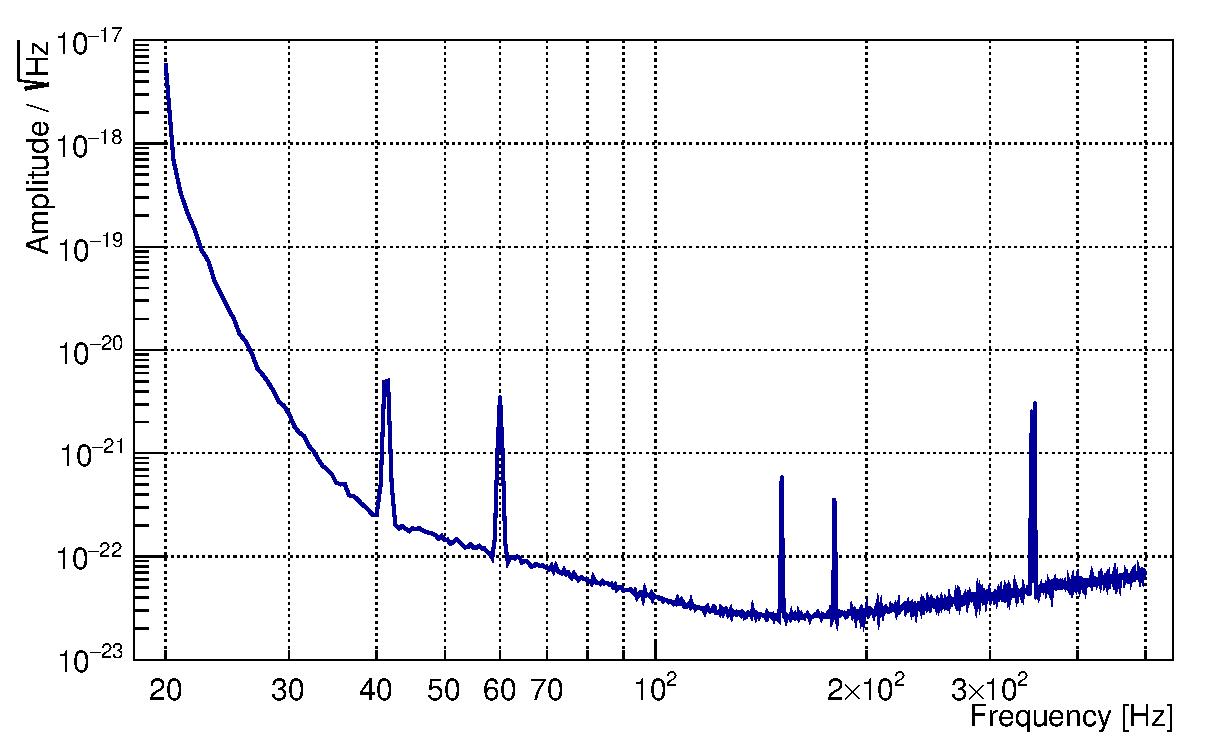
\epsfig{width=10cm, file=./figures/noise_asd.eps}
  \caption{Amplitude spectral density of simulated colored noise used to test the whitening performance of Omicron.}
  \label{fig:noise_asd}
\end{figure}
\begin{figure}
  \center
  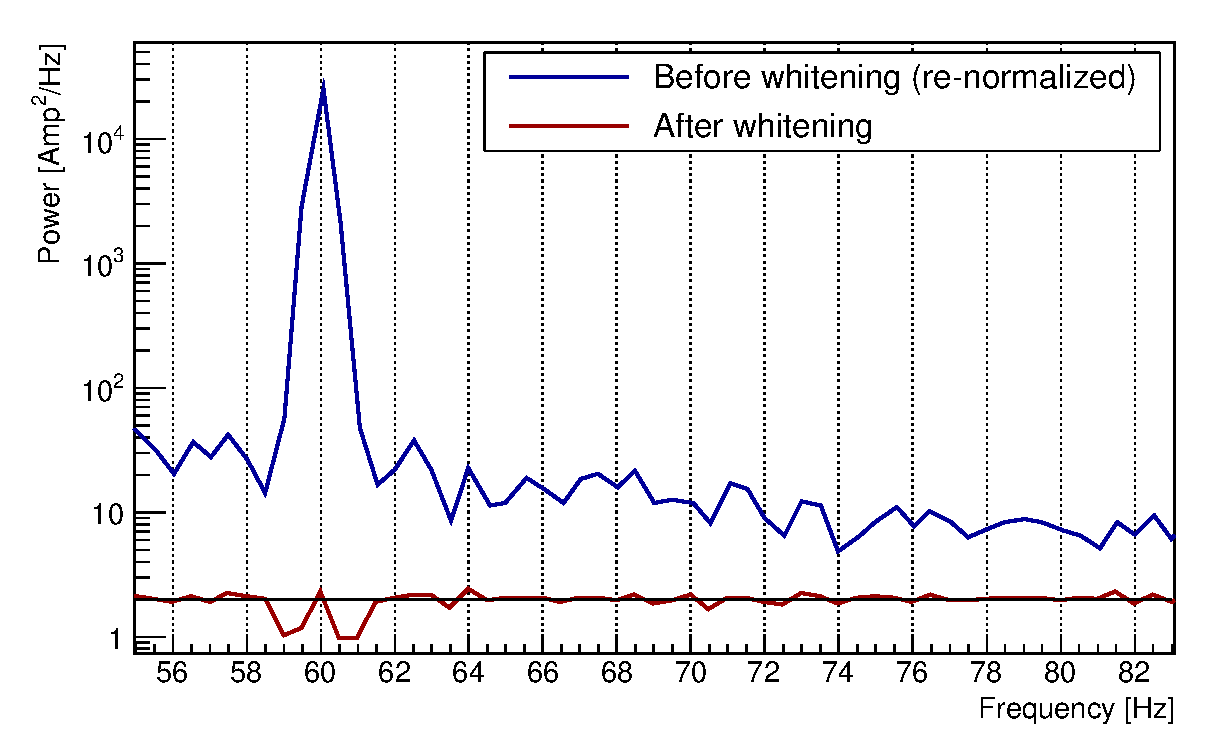
\epsfig{width=8cm, file=./figures/char_cw_line60.eps}
  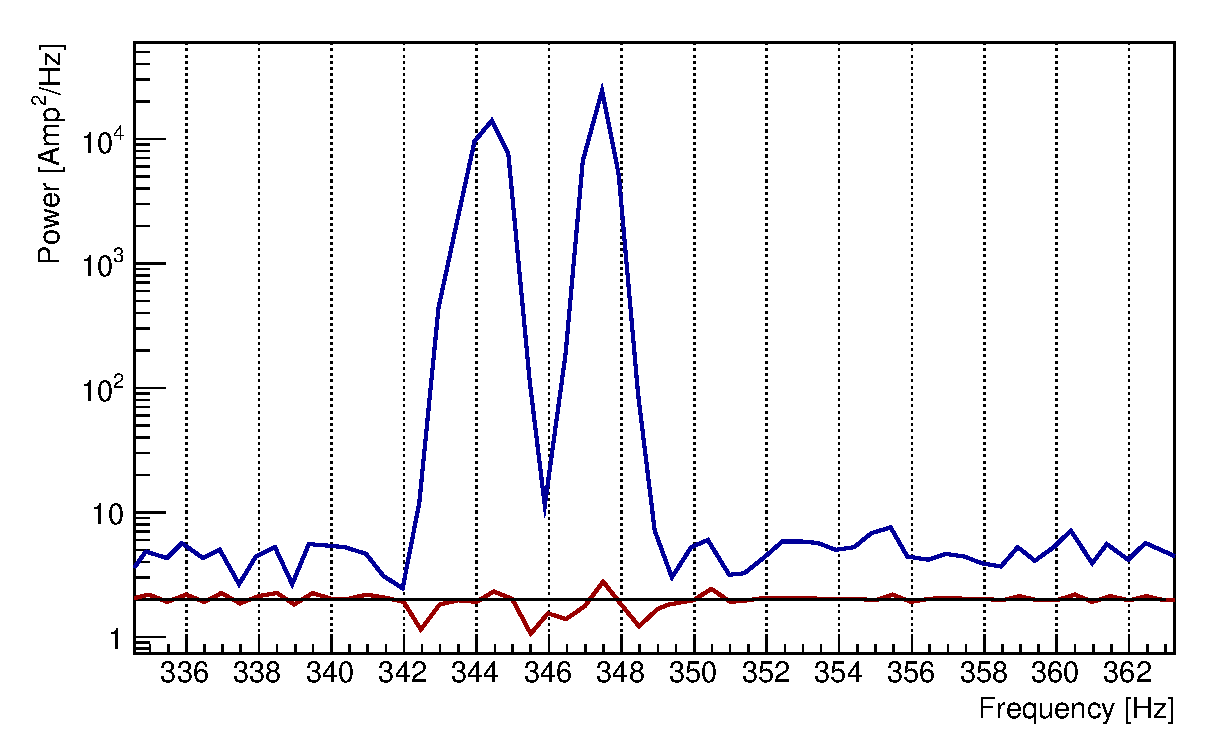
\epsfig{width=8cm, file=./figures/char_cw_line345.eps}
  \caption{Power spectral density measured by Omicron before (blue) and after (red) whitening the colored noise data set. Plots present a zoom around a single spectral line centered on 60~Hz and a line doublet around 346~Hz. The whitened spectrum is expected to be centered on 2. Around spectral lines, the noise power is overestimated and the data is over-whitened.}
  \label{fig:char_cw_line}
\end{figure}
\begin{figure}
  \center
  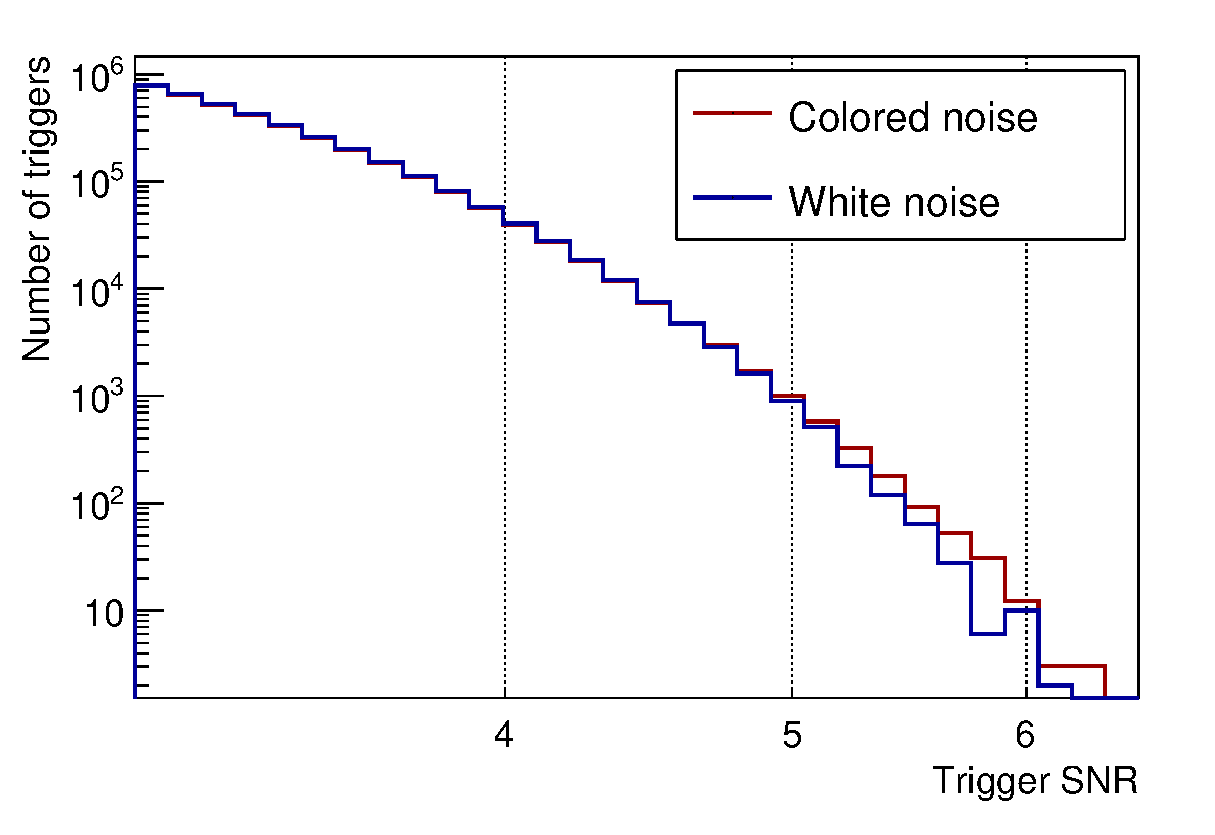
\epsfig{width=8cm, file=./figures/char_cw_snr.eps}
  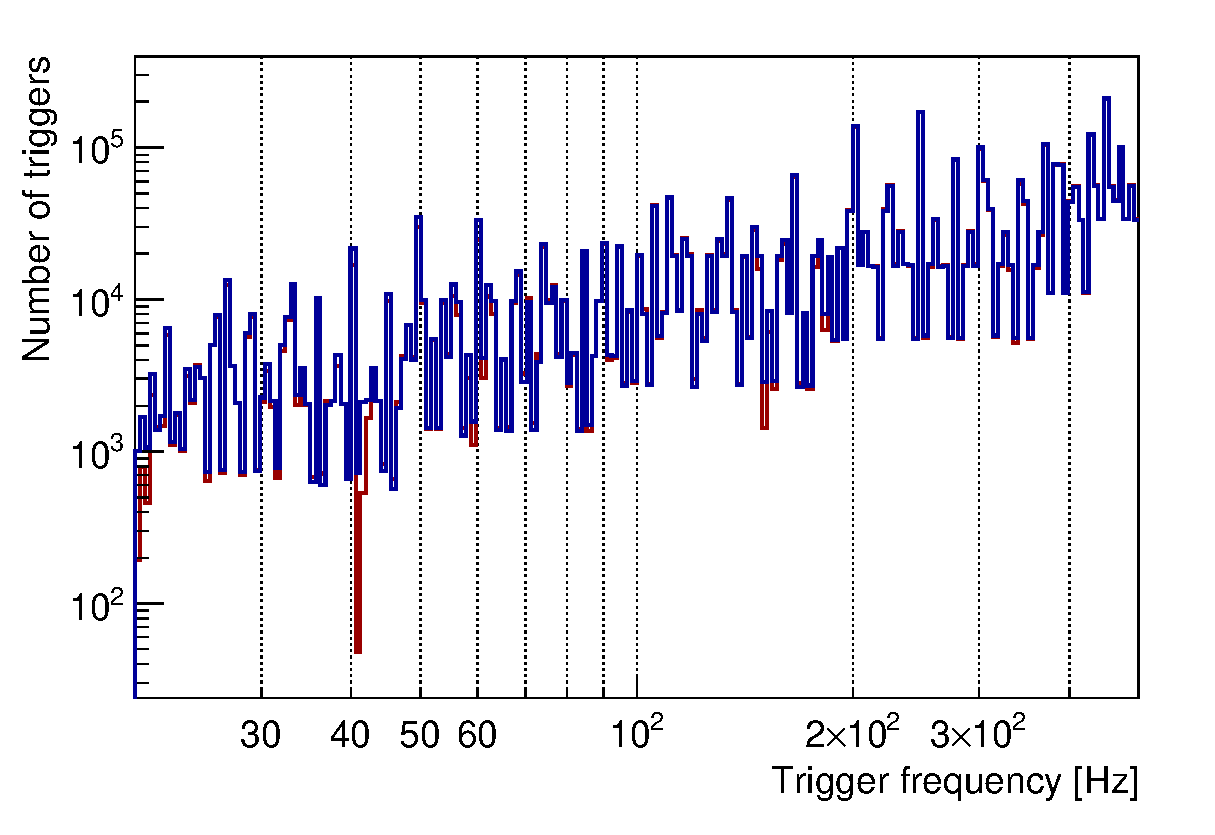
\epsfig{width=8cm, file=./figures/char_cw_freq.eps}
  \caption{Trigger SNR distribution (left) and frequency distribution (right) for colored (red) and white (blue) noise. Histograms have been normalized to get the same number of triggers in the 200-300~Hz band.}
  \label{fig:char_cw}
\end{figure}


\subsection{White noise} \label{sec:characterization:white}
In this section, the Omicron trigger generator is characterized. To achieve this, we consider Gaussian noise and, on top of it, we inject sinusoidal Gaussian burst signals with known characteristics. This is done using the injection feature of Omicron described in Sec.~\ref{sec:algorithm:injections}. The burst waveform is given in Eq.~\ref{eq:sginj}. Then, we estimate the accuracy with which Omicron recovers the signal parameters.
\begin{itemize}
\item The timing accuracy is estimated with the absolute time difference, $\tau_o-\tau_b$, where $\tau_o$ is the time measured by Omicron (tile central time) and $\tau_b$ is the time of the injection.
\item The frequency accuracy is estimated with the relative difference, $(\phi_o-\phi_b)/\phi_b$, where $\phi_o$ is the frequency measured by Omicron (tile central frequency) and $\phi_b$ is the frequency of the injection.
\item The SNR accuracy is estimated with the relative difference, $(\rho_o-\rho_b)/\rho_b$, where $\rho_o$ is the SNR estimated by Omicron (tile SNR computed with Eq.~\ref{eq:snrestimator}) and $\rho_b$ is the true SNR of the injection given by Eq.~\ref{eq:snr_white}.
\end{itemize}

As a first characterization test, we inject burst signals on top of white noise. The burst frequency $\phi_b$ and quality factor $Q_b$ take random values between 32~Hz and 256~Hz and between 4 and 64 respectively. The time of the burst is randomly drawn in $\pm10$~s around the chunk center. Signals are injected using a fix amplitude $B$ such that the resulting true SNR is $\rho_b=10$. Then we run Omicron with the parameters listed in Appx~\ref{appx:parameters} over a data set containing 1038 burst injections. The maximal fractional energy loss between tiles is varied around the nominal value of $\mu_{max}=20\%$ and the resulting recovery histograms for SNR, time and frequency are displayed in Fig.~\ref{fig:char_mismatch}. The SNR recovery histogram is well compatible with the Monte Carlo study presented in Fig.~\ref{fig:snrestimator} and Tab.~\ref{tab:snrestimator}. The mean value for the $\mu_{max}=5\%$ distribution is -0.8\% while it was predicted to be -0.51\% when the match between the tile and the signal is perfect. The standard deviation for $\mu_{max}=20\%$ is $\pm9.95\%$ while it was found to be $\pm10.08\%$ with Monte Carlo studies. The time and frequency recovery histograms are well centered on 0 proving that Omicron does not introduce any bias. Omicron adopts a multi-resolution tiling structure (see Sec.~\ref{sec:algorithm:tiling}): the time and frequency resolution is a function of the frequency and the quality factor. Fig.~\ref{fig:char_mismatch} show that, in average, for the injection parameter ranges chosen above and for $\mu_{max}=20\%$, the timing is recovered with a $\pm8$~ms precision and the frequency is resolved at $\pm2.4\%$. 
\begin{figure}
  \center
  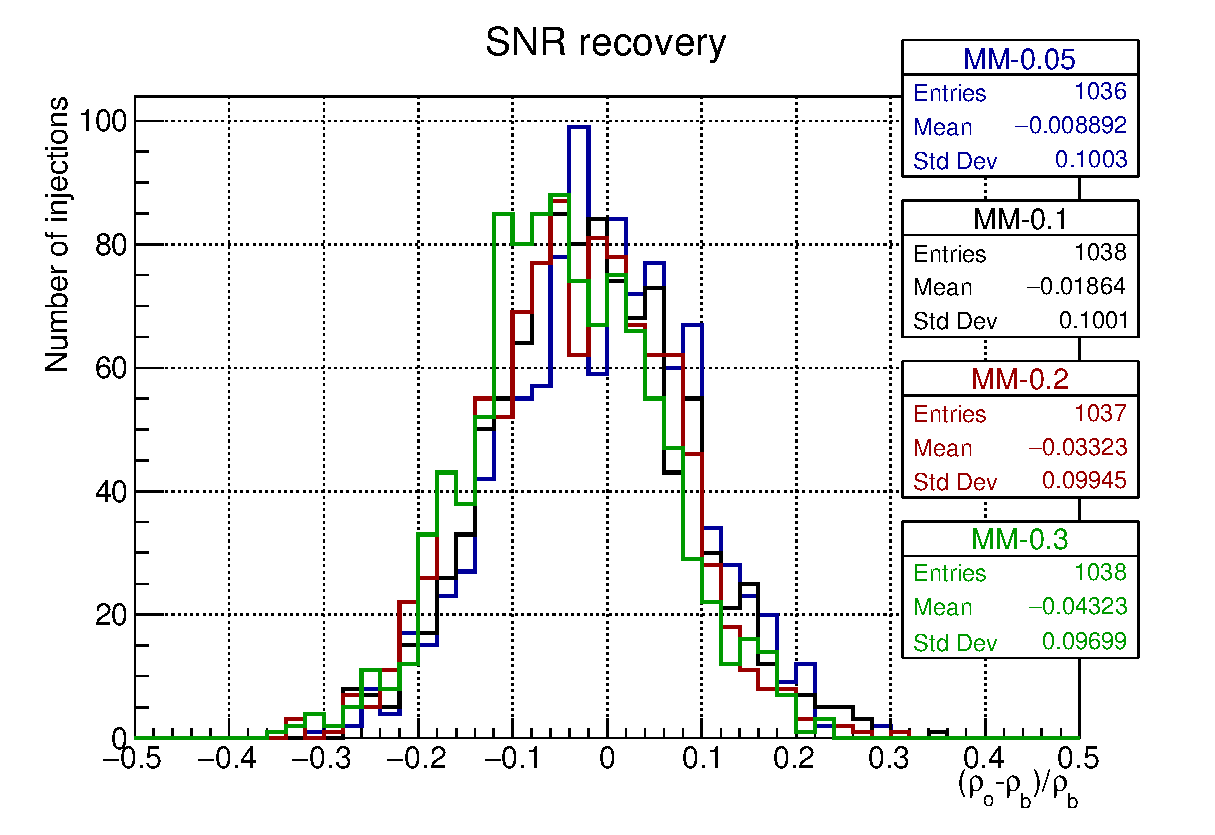
\epsfig{width=8.5cm, file=./figures/char_mismatch_snr.eps}
  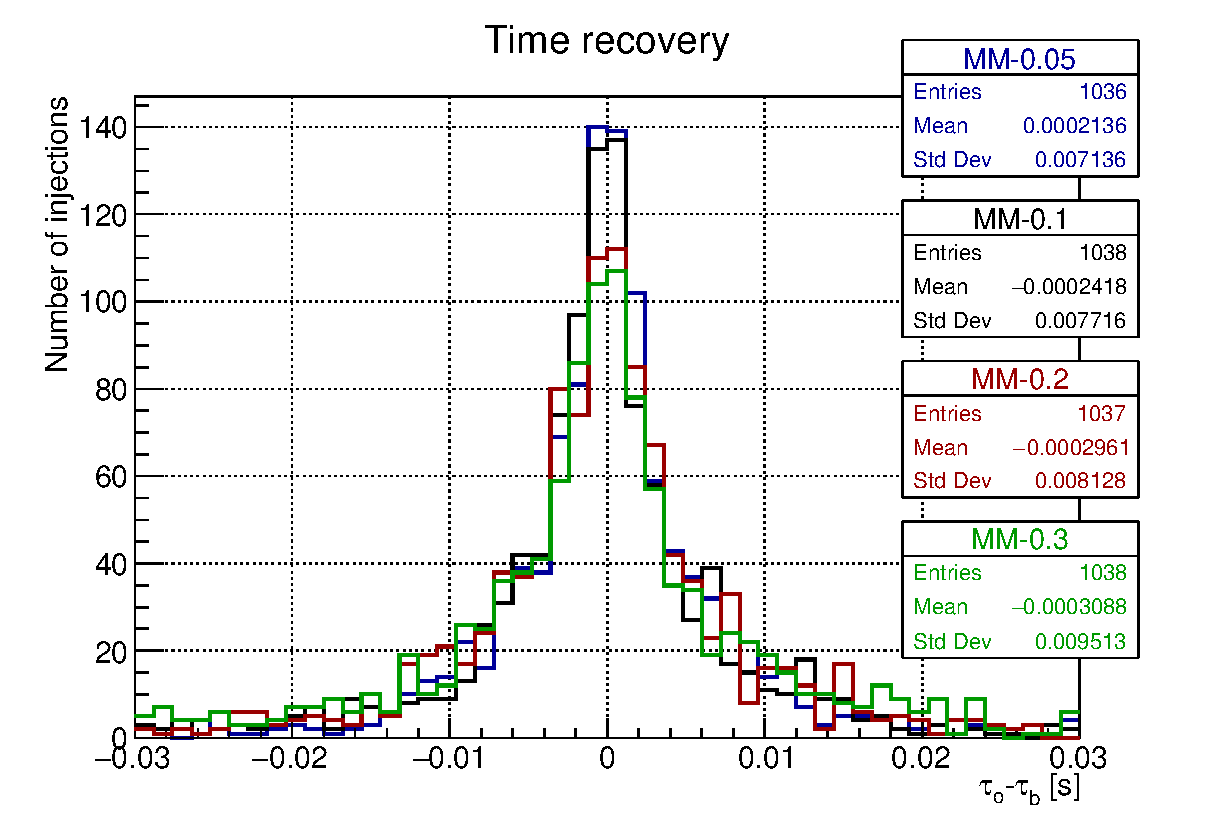
\epsfig{width=8.5cm, file=./figures/char_mismatch_time.eps} \\
  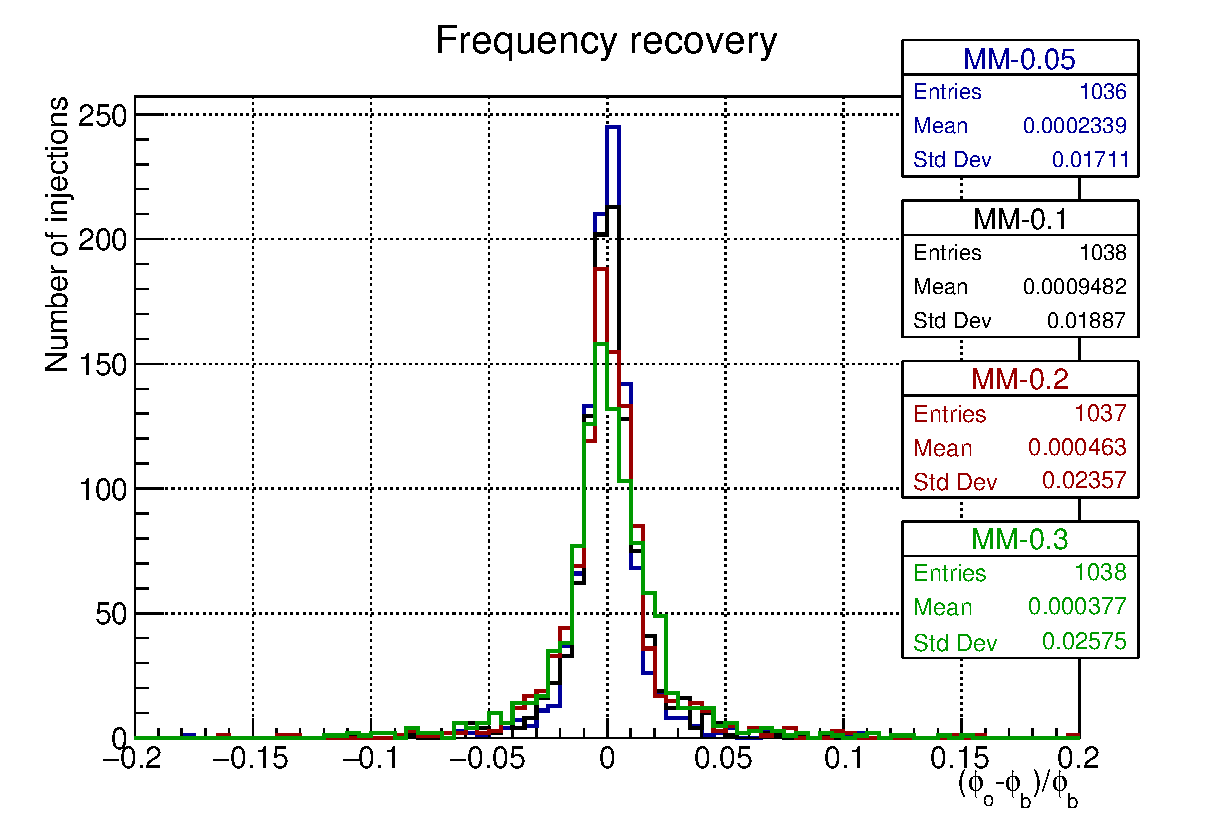
\epsfig{width=8.5cm, file=./figures/char_mismatch_freq.eps}
  \caption{Omicron SNR, time and frequency reconstruction performance as a function of the maximal fractional energy loss between tiles, $\mu_{max}$. Four values of $\mu_{max}$ were used: 5\% (blue), 10\% (black), 20\% (red) and 30\% (green). The distribution mean values and standard deviations are reported in the color boxes.}
  \label{fig:char_mismatch}
\end{figure}

Now, we fix the $\mu_{max}$ parameter to 20\% and we choose discrete values for the quality factor of the injections: $Q_b=4$, $Q_b=16$, $Q_b=32$ and $Q_b=64$. Fig.~\ref{fig:char_q} shows how Omicron recovers the signal parameters for these four data sets. The SNR parameter recovery is independent from the $Q$ value. As expected (see Eqs.~\ref{eq:sigf} and~\ref{eq:sigt}), the frequency resolution is inversely proportional to $Q$ and the time resolution is proportional to $Q$.
\begin{figure}
  \center
  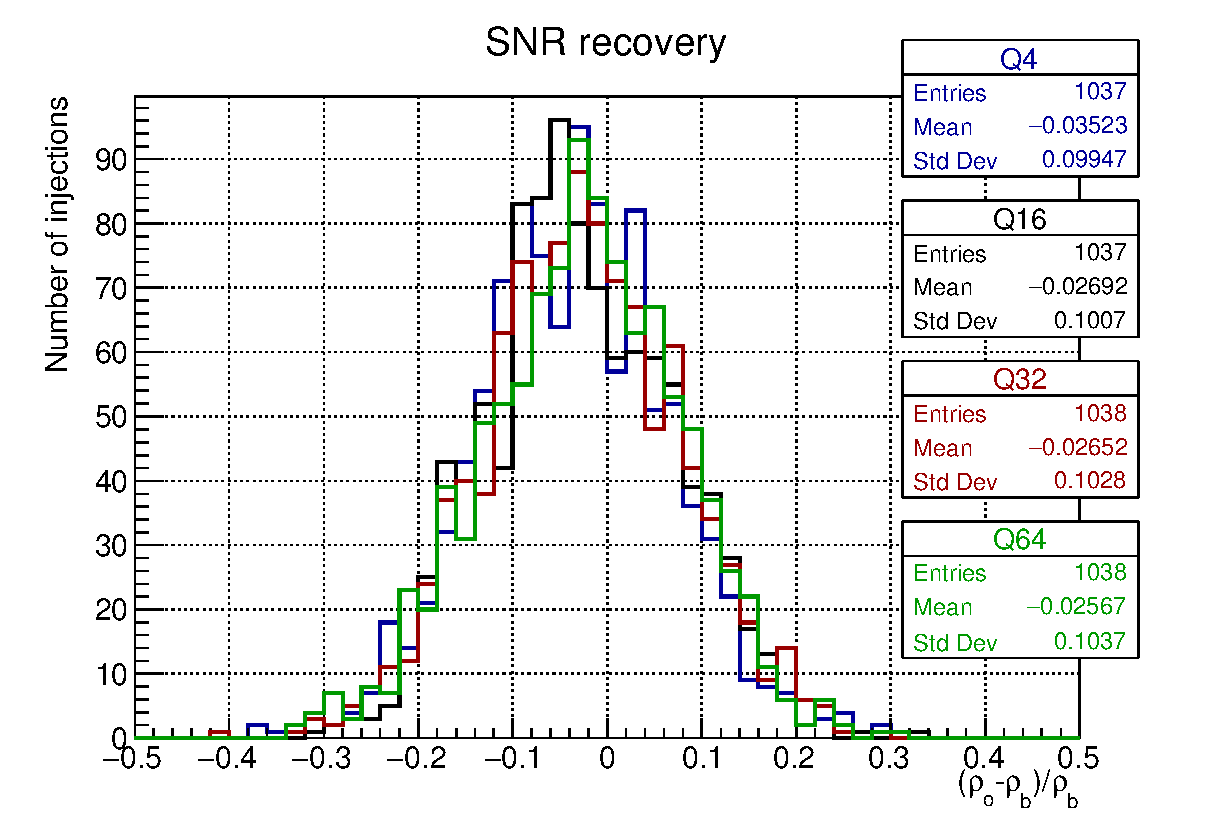
\epsfig{width=8.5cm, file=./figures/char_Q_snr.eps}
  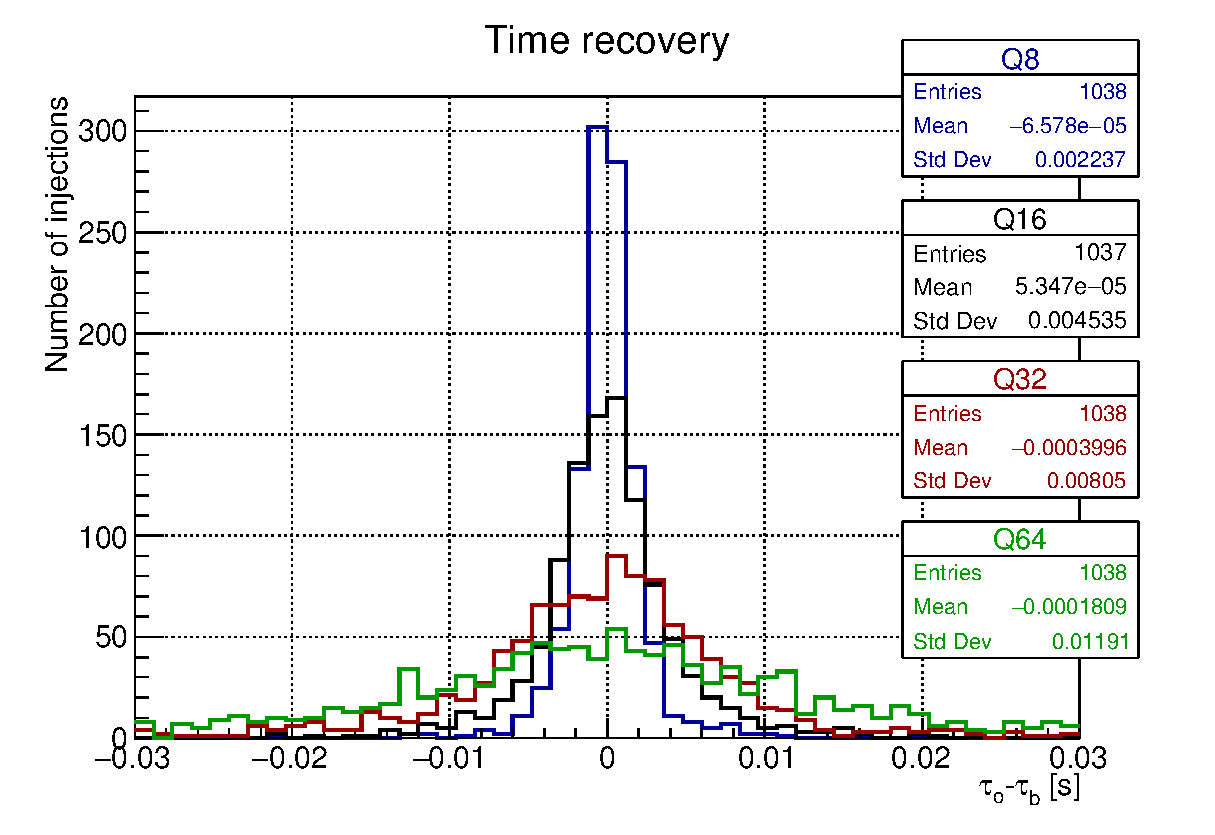
\epsfig{width=8.5cm, file=./figures/char_Q_time.eps} \\
  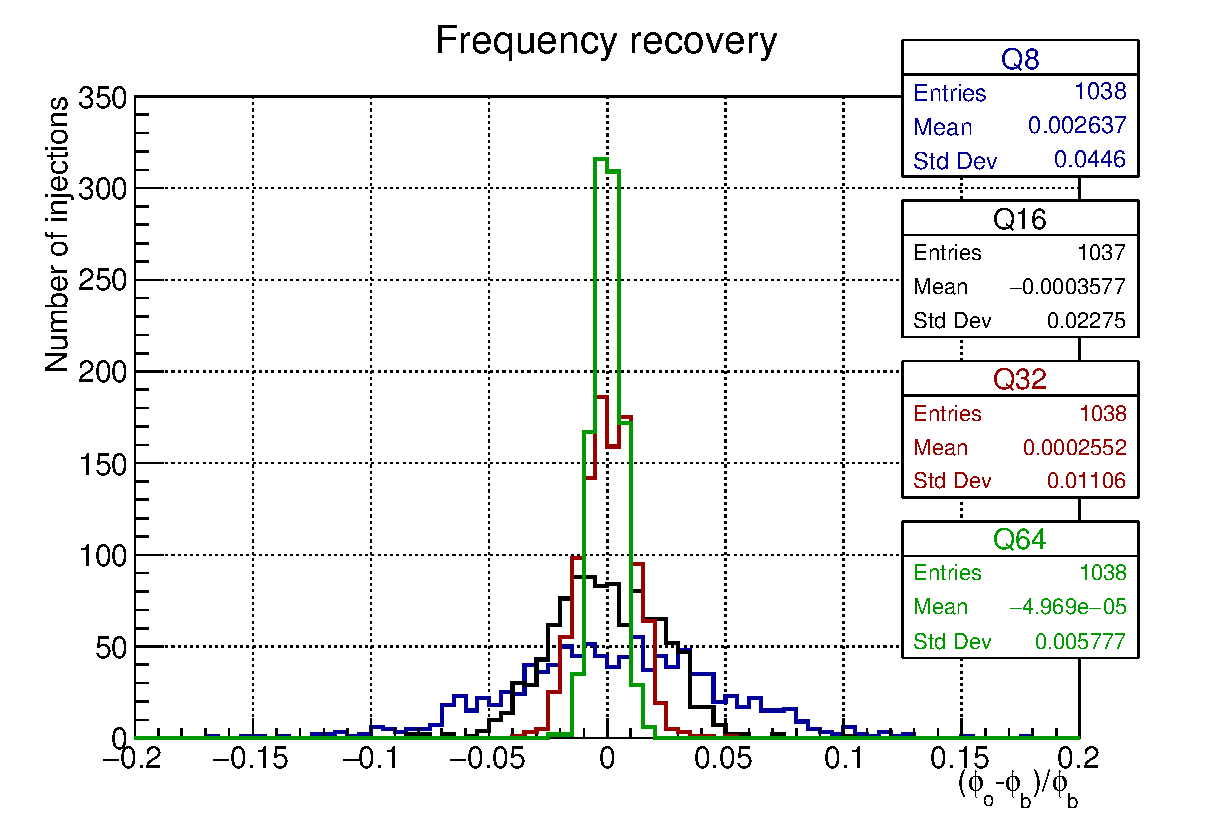
\epsfig{width=8.5cm, file=./figures/char_Q_freq.eps}
  \caption{Omicron SNR, time and frequency reconstruction performance as a function of the signal quality factor, $Q_b$. Four values of $Q_b$ were used: 8 (blue), 16 (black), 32 (red) and 64 (green). The distribution mean values and standard deviations are reported in the color boxes.}
  \label{fig:char_q}
\end{figure}

Now, all the injection parameters are set free: $4<Q_b<64$, 32~Hz$<\phi_b<$256~Hz, and $2.5<\rho_b<250$. For this injection set, the Omicron performance are estimated and plotted in Figs.~\ref{fig:char_snr},~\ref{fig:char_time} and~\ref{fig:char_freq}
\begin{figure}
  \center
  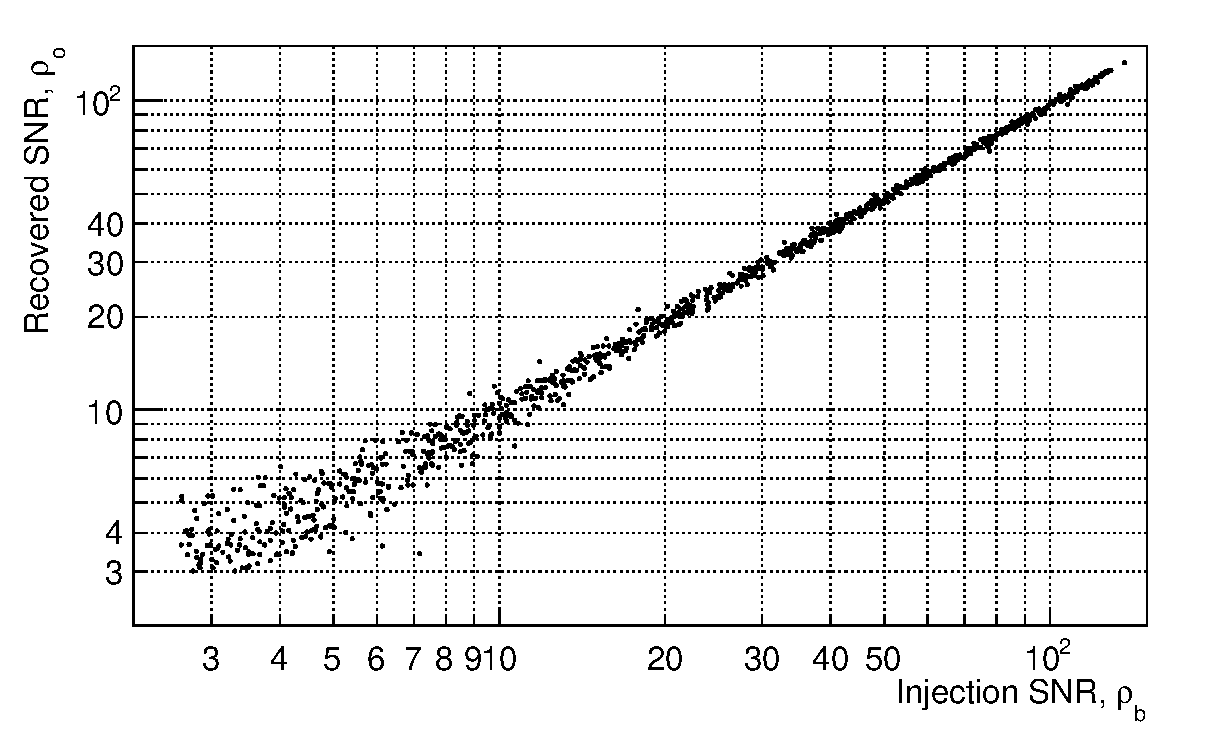
\epsfig{width=8.5cm, file=./figures/char_snrsnr.eps} \\
  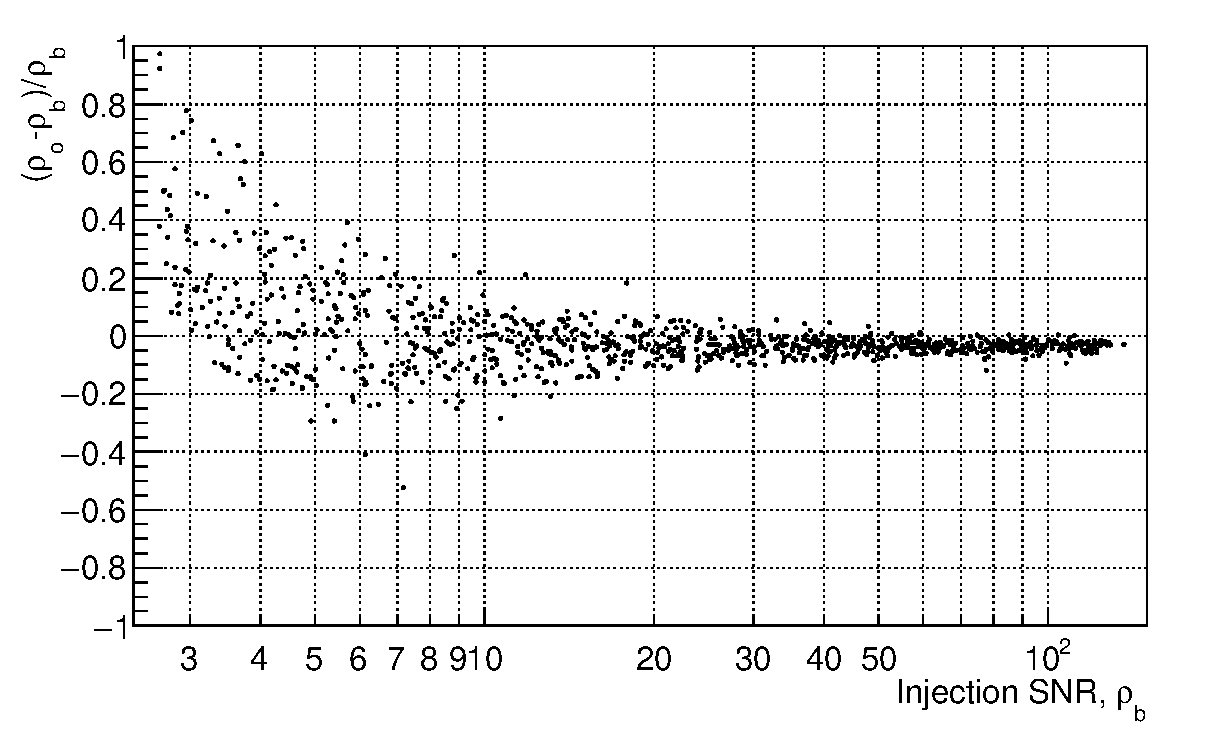
\epsfig{width=8.5cm, file=./figures/char_rsnrsnr.eps}
  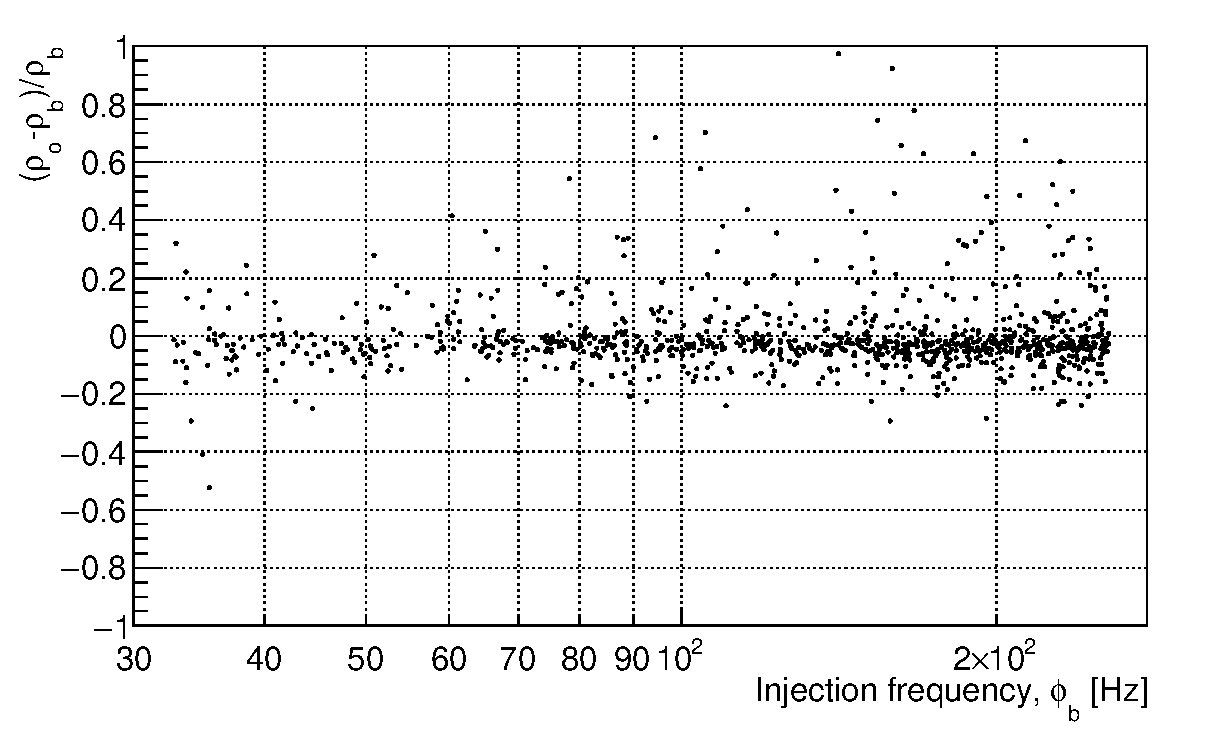
\epsfig{width=8.5cm, file=./figures/char_rsnrfreq.eps}
  \caption{Omicron SNR reconstruction performance as a function of the signal SNR and frequency. The top plot shows the recovered SNR $\rho_o$ as a function of the injection SNR $\rho_b$. The bottom plots show the relative SNR difference as a function of the injection SNR $\rho_b$ (left) and the injection frequency $\phi_b$ (right).}
  \label{fig:char_snr}
\end{figure}

\begin{figure}
  \center
  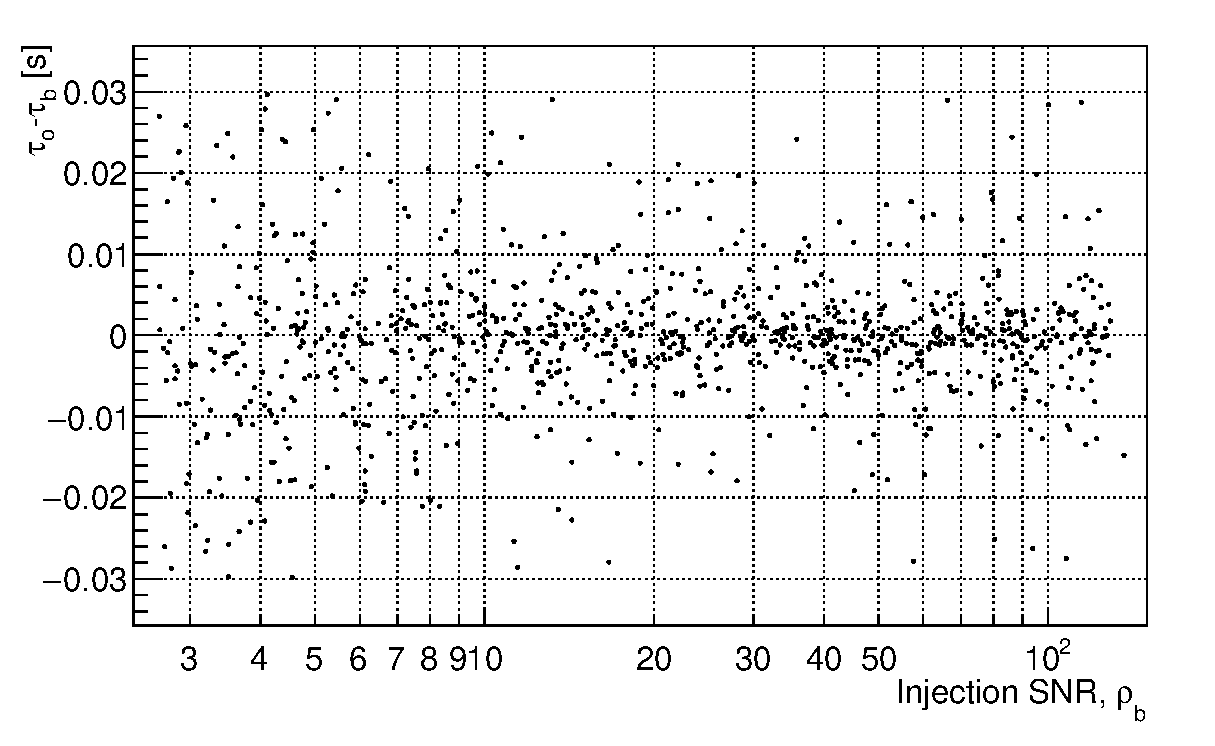
\epsfig{width=8.5cm, file=./figures/char_dtsnr.eps}
  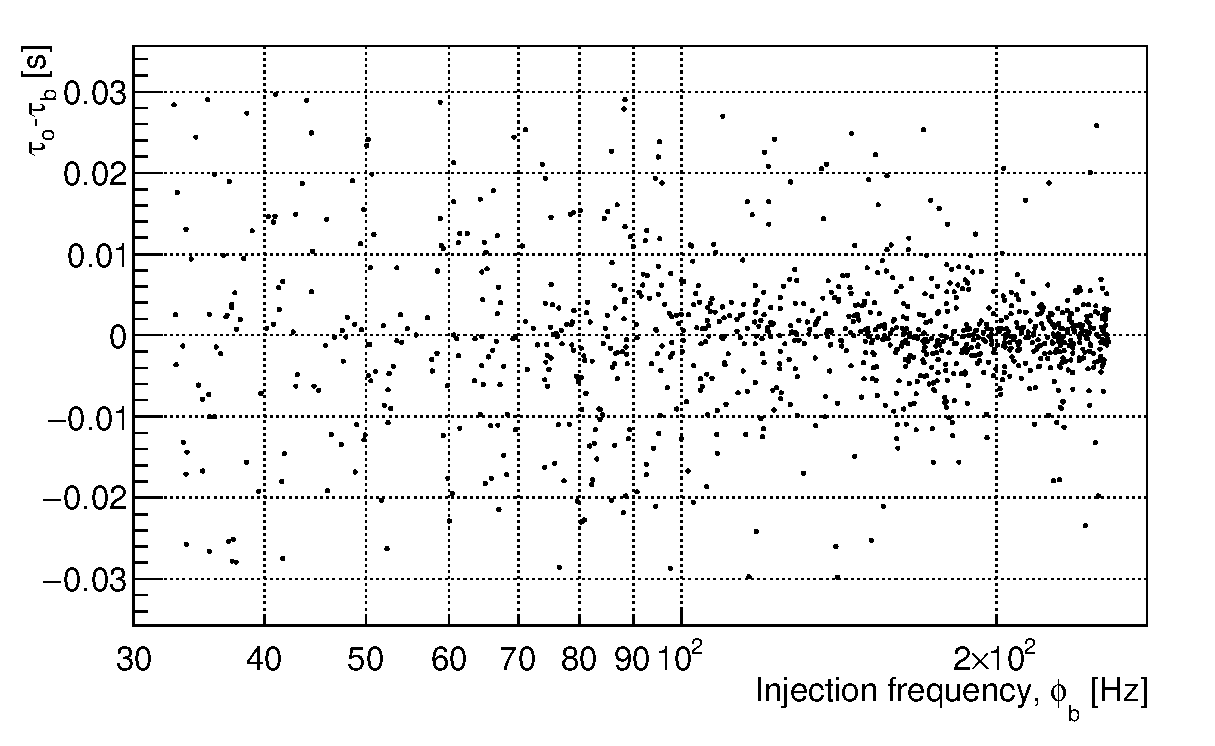
\epsfig{width=8.5cm, file=./figures/char_dtfreq.eps}
  \caption{Omicron time reconstruction performance as a function of the signal SNR and frequency. The plots show the absolute time difference between the recovered event and the injection, $\tau_o-\tau_b$, as a function of the injection SNR $\rho_b$ (left) and the injection frequency $\phi_b$ (right).}
  \label{fig:char_time}
\end{figure}


\begin{figure}
  \center
  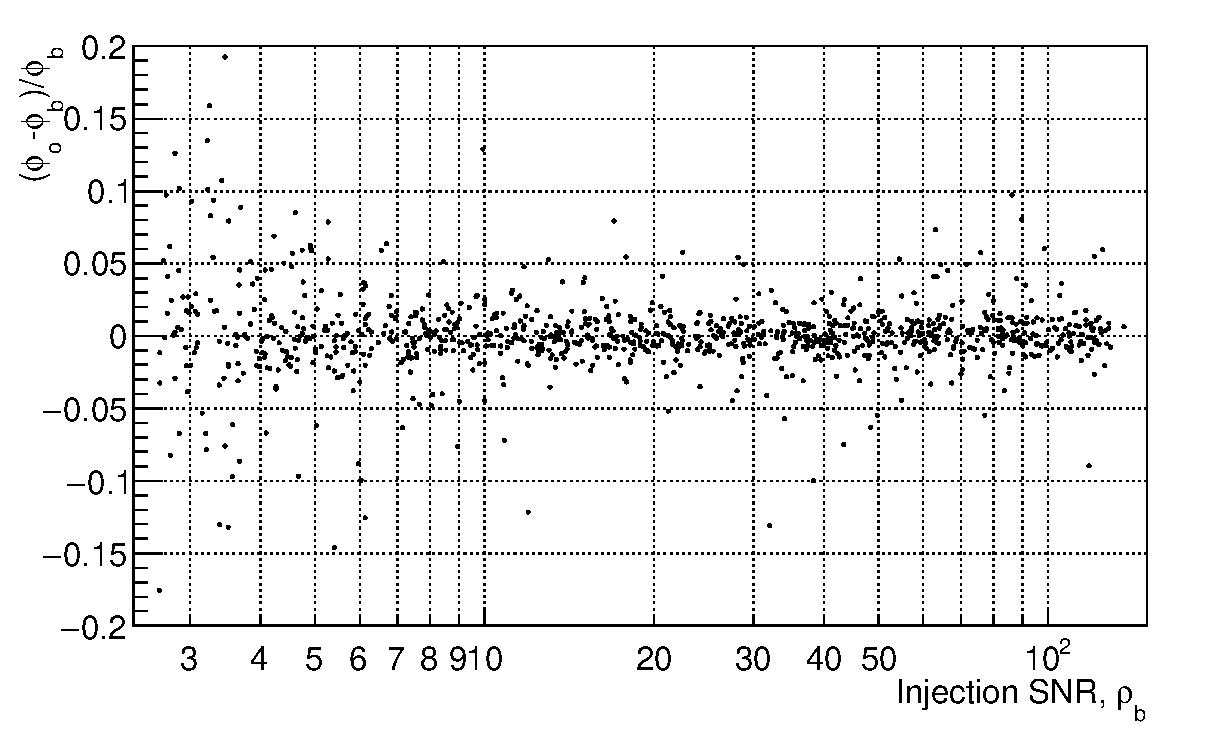
\epsfig{width=8.5cm, file=./figures/char_rfsnr.eps}
  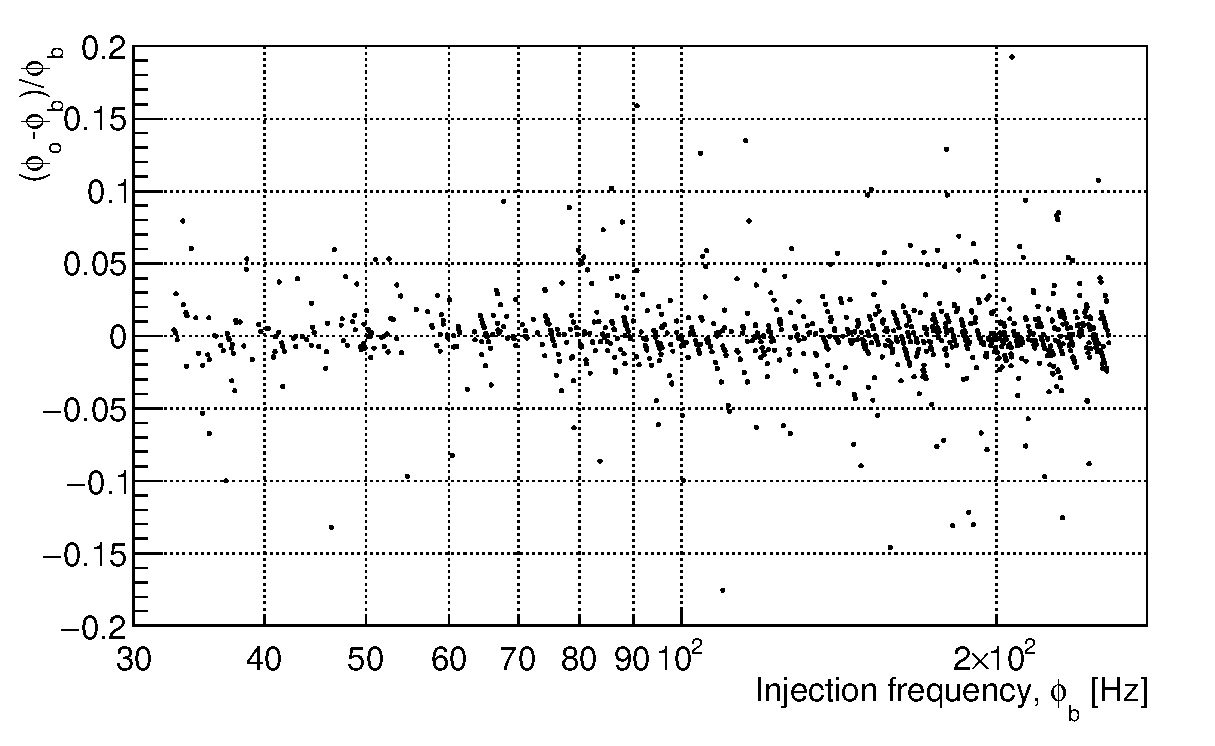
\epsfig{width=8.5cm, file=./figures/char_rffreq.eps}
  \caption{Omicron frequency reconstruction performance as a function of the signal SNR and frequency. The plots show the relative frequency difference between the recovered event and the injection, $\phi_o-\phi_b$, as a function of the injection SNR $\rho_b$ (left) and the injection frequency $\phi_b$ (right).}
  \label{fig:char_freq}
\end{figure}
